%% Coordenadas Esf'ericas.
%% Adaptado por Regis da Silva Santos
%% latexbr.blogspot.com.br
%% Stereographic and cylindrical map projections
%% Author: Tomasz M. Trzeciak
%% Source: LaTeX-Community.org
%%         <http://www.latex-community.org/viewtopic.php?f=4&t=2111>
%%
\documentclass[tikz]{standalone}
\usepackage{tikz}
\usetikzlibrary{calc,fadings,decorations.pathreplacing}

%% helper macros

\newcommand\pgfmathsinandcos[3]{%
  \pgfmathsetmacro#1{sin(#3)}%
  \pgfmathsetmacro#2{cos(#3)}%
}
\newcommand\LongitudePlane[3][current plane]{%
  \pgfmathsinandcos\sinEl\cosEl{#2} % elevation
  \pgfmathsinandcos\sint\cost{#3} % azimuth
  \tikzset{#1/.estyle={cm={\cost,\sint*\sinEl,0,\cosEl,(0,0)}}}
}
\newcommand\LatitudePlane[3][current plane]{%
  \pgfmathsinandcos\sinEl\cosEl{#2} % elevation
  \pgfmathsinandcos\sint\cost{#3} % latitude
  \pgfmathsetmacro\yshift{\cosEl*\sint}
  \tikzset{#1/.estyle={cm={\cost,0,0,\cost*\sinEl,(0,\yshift)}}} %
}
\newcommand\DrawLongitudeCircle[2][1]{
  \LongitudePlane{\angEl}{#2}
  \tikzset{current plane/.prefix style={scale=#1}}
   % angle of "visibility"
  \pgfmathsetmacro\angVis{atan(sin(#2)*cos(\angEl)/sin(\angEl))} %
  \draw[current plane] (\angVis:1) arc (\angVis:\angVis+180:1);
  \draw[current plane,dashed] (\angVis-180:1) arc (\angVis-180:\angVis:1);
}
\newcommand\DrawLatitudeCircle[2][1]{
  \LatitudePlane{\angEl}{#2}
  \tikzset{current plane/.prefix style={scale=#1}}
  \pgfmathsetmacro\sinVis{sin(#2)/cos(#2)*sin(\angEl)/cos(\angEl)}
  % angle of "visibility"
  \pgfmathsetmacro\angVis{asin(min(1,max(\sinVis,-1)))}
  \draw[current plane] (\angVis:1) arc (\angVis:-\angVis-180:1);
  \draw[current plane,dashed] (180-\angVis:1) arc (180-\angVis:\angVis:1);
}

%%% document-wide tikz options and styles

\tikzset{%
  >=latex, % option for nice arrows
  inner sep=0pt,%
  outer sep=2pt,%
  mark coordinate/.style={inner sep=0pt,outer sep=0pt,minimum size=3pt,
    fill=black,circle}%
}

\begin{document}

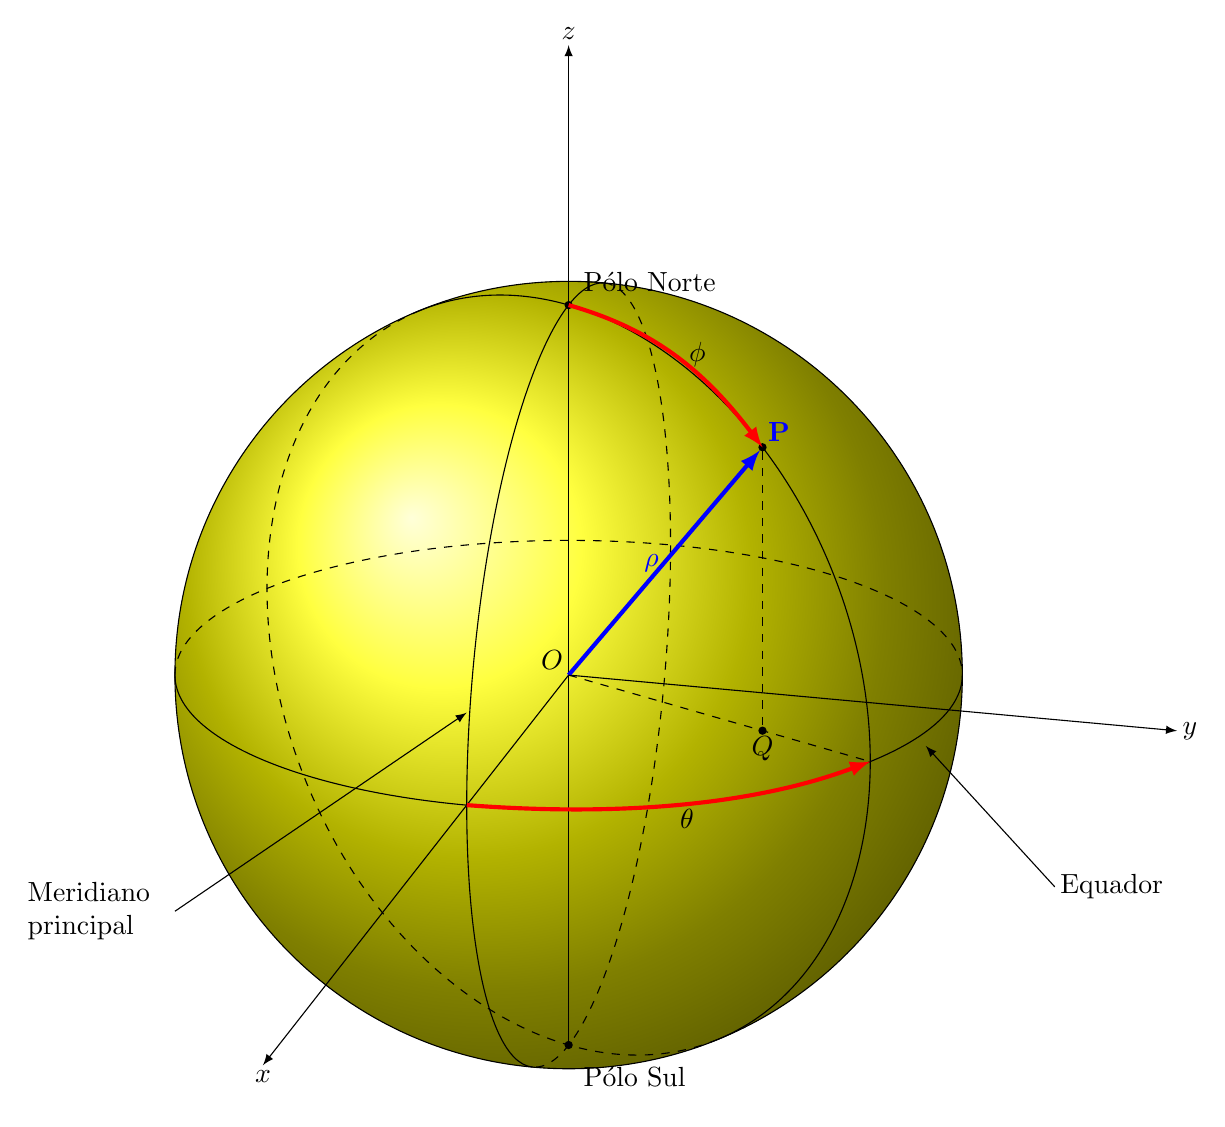
\begin{tikzpicture}[scale=2]

%% some definitions

\def\R{2.5} % sphere radius
\def\angEl{20} % elevation angle
\def\angAz{-105} % azimuth angle
\def\angPhi{-40} % longitude of point P
\def\angBeta{50} % latitude of point P

%% working planes

\pgfmathsetmacro\H{\R*cos(\angEl)} % distance to north pole
\pgfmathsetmacro\Q{\R*cos(\angBeta)} % dist�ncia do ponto Q
\tikzset{xyplane/.estyle={cm={cos(\angAz),sin(\angAz)*sin(\angEl),-sin(\angAz),
                              cos(\angAz)*sin(\angEl),(0,0)}}}
\LongitudePlane[xzplane]{\angEl}{\angAz}
\LongitudePlane[pzplane]{\angEl}{\angPhi}
\LatitudePlane[equator]{\angEl}{0}

%% draw xyplane and sphere

%\draw[xyplane] (-2*\R,-2*\R) rectangle (2.2*\R,2.8*\R);
\fill[ball color=yellow] (0,0) circle (\R); % 3D lighting effect
\draw (0,0) circle (\R);

%% characteristic points

\coordinate (O) at (0,0);
\coordinate[mark coordinate] (N) at (0,\H);
\coordinate[mark coordinate] (S) at (0,-\H);
\path[pzplane] (\angBeta:\R) coordinate[mark coordinate] (P);
\path[pzplane] (\R,0) coordinate (PE);
\path[xzplane] (\R,0) coordinate (XE);
%\path (PE) ++(0,-\H) coordinate (Paux); % to aid Phat calculation
%\coordinate[mark coordinate] (Phat) at (intersection cs: first line={(N)--(P)},
%                                        second line={(S)--(Paux)});
\path[pzplane] (\Q,0) coordinate[mark coordinate] (Q); %defini��o do ponto Q

%% draw meridians and latitude circles

\DrawLatitudeCircle[\R]{0} % equator
%\DrawLatitudeCircle[\R]{\angBeta}
\DrawLongitudeCircle[\R]{\angAz} % xzplane
%\DrawLongitudeCircle[\R]{\angAz+90} % yzplane
\DrawLongitudeCircle[\R]{\angPhi} % pzplane

%% draw xyz coordinate system

\draw[xyplane,<->] (3*\R,0) node[below] {$x$} -- (0,0) -- (0,1.6*\R)
    node[right] {$y$};
\draw[->] (0,-\H) -- (0,1.6*\R) node[above] {$z$};

%% draw lines and put labels
\path (O) node[above left] {$O$};
\path (N) +(0.4ex,-0.4ex) node[above=12pt,right] {P\'olo Norte};
\path (S) +(0.4ex,-0.4ex) node[below=8pt,right] {P\'olo Sul};
\draw[->,line width=1.5pt,color=blue] (O) -- node[midway,left] {$\rho$} (P) node[above right] {$\mathbf{P}$};
\draw[dashed] (P) -- (Q) node[below] {$Q$}; %proje��o de P sobre Q
\draw[dashed] (O) -- (PE);
\draw[pzplane,<-,line width=1.5pt,color=red] (\angBeta:\R) to[bend right=20]
    node[pos=0.5,right=4pt,color=black] {$\phi$} (90:\R);
\draw[equator,->,line width=1.5pt,color=red] (\angAz:\R) to[bend right=30]
    node[pos=0.5,below,color=black] {$\theta$} (\angPhi:\R);
\path (XE) ++(0,0.25*\H) coordinate (XEN); % to aid XEN calculation
\draw[->] (-2.5,-1.5) node[left,text width=1.8cm] {Meridiano principal} -- (XEN);
\path (PE) ++(0.15*\H,0.1) coordinate (PEN); % to aid PEN calculation
\draw[xyplane,->] (3,4) node[right] {Equador} -- (PEN);
\end{tikzpicture}
\end{document} 